\documentclass[a0paper,landscape,fontscale=0.32]{baposter}

\usepackage{relsize}		% For \smaller
\usepackage{epstopdf}	% Included EPS files automatically converted to PDF to include with pdflatex
\usepackage{float}
\usepackage{lipsum}
\usepackage{wrapfig}
\usepackage{minted}
\usepackage[none]{hyphenat}
\usepackage[sfdefault]{roboto}  %% Option 'sfdefault' only if the base font of the document is to be sans serif
\usepackage[T1]{fontenc}
\usepackage{multicol}

\usepackage{tcolorbox}
\BeforeBeginEnvironment{minted}{\begin{tcolorbox}}%
\AfterEndEnvironment{minted}{\end{tcolorbox}}%

\usemintedstyle{autumn}

\usepackage{enumitem}
\setlist[itemize]{leftmargin=*,itemsep=0pt}

\renewcommand\fbox{\fcolorbox{blue}{white}}
\setlength{\fboxsep}{0pt}
\setlength{\fboxrule}{5pt}

%%% Global Settings %%%%%%%%%%%%%%%%%%%%%%%%%%%%%%%%%%%%%%%%%%%%%%%%%%%%%%%%%%%

\graphicspath{{pix/}}	% Root directory of the pictures
\tracingstats=2			% Enabled LaTeX logging with conditionals

%%%%%%%%%%%%%%%%%%%%%%%%%%%%%%%%%%%%%%%%%%%%%%%%%%%%%%%%%%%%%%%%%%%%%%%%%%%%%%%%
%%% Utility functions %%%%%%%%%%%%%%%%%%%%%%%%%%%%%%%%%%%%%%%%%%%%%%%%%%%%%%%%%%

%%% Save space in lists. Use this after the opening of the list %%%%%%%%%%%%%%%%
\newcommand{\compresslist}{
	\setlength{\itemsep}{1pt}
	\setlength{\parskip}{0pt}
	\setlength{\parsep}{0pt}
}

%%%%%%%%%%%%%%%%%%%%%%%%%%%%%%%%%%%%%%%%%%%%%%%%%%%%%%%%%%%%%%%%%%%%%%%%%%%%%%%
%%% Document Start %%%%%%%%%%%%%%%%%%%%%%%%%%%%%%%%%%%%%%%%%%%%%%%%%%%%%%%%%%%%
%%%%%%%%%%%%%%%%%%%%%%%%%%%%%%%%%%%%%%%%%%%%%%%%%%%%%%%%%%%%%%%%%%%%%%%%%%%%%%%

\begin{document}
\typeout{Poster rendering started}

%%% Setting Background Image %%%%%%%%%%%%%%%%%%%%%%%%%%%%%%%%%%%%%%%%%%%%%%%%%%
\background{template.svg}

%%% General Poster Settings %%%%%%%%%%%%%%%%%%%%%%%%%%%%%%%%%%%%%%%%%%%%%%%%%%%
%%%%%% Eye Catcher, Title, Authors and University Images %%%%%%%%%%%%%%%%%%%%%%
\begin{poster}{
	grid=false,
	% Option is left on true though the eyecatcher is not used. The reason is
	% that we have a bit nicer looking title and author formatting in the headercol
	% this way
	eyecatcher=true,
	borderColor=blue,
	headerColorOne=blue,
	headerColorTwo=blue,
	headerFontColor=white,
	headerborder=closed,
	% Only simple background color used, no shading, so boxColorTwo isn't necessary
	boxColorOne=white,
	headershape=smallrounded,
	headerborder=open,
	headerfont=\Large\sf\bf,
	textborder=rectangle,
	background=none,
    boxshade=plain,
    columns=4
}
%%% Title %%%%%%%%%%%%%%%%%%%%%%%%%%%%%%%%%%%%%%%%%%%%%%%%%%%%%%%%%%%%%%%%%%%%%
{
\includegraphics[height=4em]{images/diamondlogo}}
{\bf \color{blue} Syringe Pump for Electrochemical Cell \vspace{0.5em}} % Poster title
{\textbf{Dolica Akello-Egwel}, Gary Yendell \hspace{12pt} 2018 Cohort / Mantid Team} % Author names and institution
{
\includegraphics[height=4em]{images/stfclogo}}

%%%% Column 1 %%%%%%%%%%%%%%%%%%%%%%%%%%%%%%%%%%%%%%%%%%%%%%%%%%%%%%%%%%%%%%%%%%
%----------------------------------------------------------------------------------------
%	INTRODUCTION
%----------------------------------------------------------------------------------------
\begin{posterbox}[name=introduction,column=0]{Introduction}
The existing streamDevice-based EPICS driver for the Hamilton Microlab 500/600 Syringe Pump was not
especially suited to sending "complex" commands that contain two or more instructions.
The driver also lacked the ability to reliably send simultaneous commands to both syringes, and to
cycle sets of simultaneous commands indefinetly. The aim of this project was to create a user-friendly
and extensible Python API that addresses these issues and enables users to easily create continuous flows
through an electrochemical cell.
\begin{figure}[H]
\begin{center}
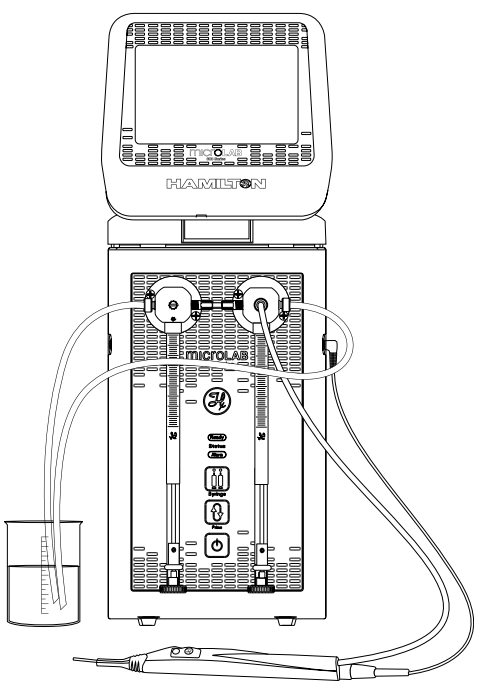
\includegraphics[width=100pt]{images/syringediagram}
\caption{Diagram of the syringe pump}
\end{center}
\end{figure}
\end{posterbox}
%----------------------------------------------------------------------------------------
%	OBJECTIVES
%----------------------------------------------------------------------------------------
\begin{posterbox}[name=objectives,column=0,row=0,below=introduction]{Objectives}
 \begin{itemize}
    \item Make a Python library for controlling the Hamilton Microlab Syringe Pump
    \item Allow the library to be controlled with a command-line interface
    \item Add a cycling ability to allow the manipulation of continuous flows
    \item Allow the syringe paramters to be controlled via EPICS
    \item Create a graphical interface using EDM screens
\end{itemize}
\end{posterbox}
%----------------------------------------------------------------------------------------
%	REMOTE WORK
%----------------------------------------------------------------------------------------
\setlength{\fboxrule}{0.8pt}
\begin{posterbox}[name=remotework,column=0,headerfont={},headershape=rounded,boxheaderheight=0em,borderColor=white,below=objectives]{}
\begin{figure}[H]
\begin{center}
\vspace{-1.8em}
\setlength{\fboxrule}{2pt}
\fbox{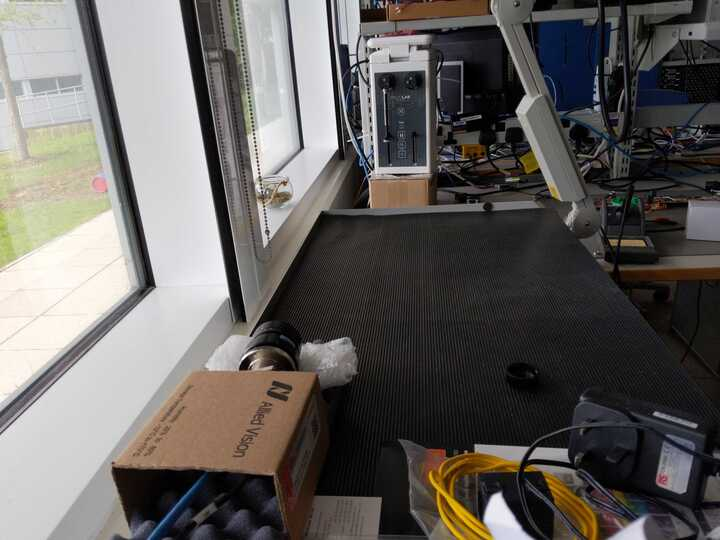
\includegraphics[width=0.7\textwidth]{images/camerasetup}}
\caption{Remote working setup: a GigE camera is facing the syringe, and the camera feed is streamed through http.}
\vspace{-1.2em}
\end{center}
\end{figure}
\end{posterbox}

%%%% Column 2 %%%%%%%%%%%%%%%%%%%%%%%%%%%%%%%%%%%%%%%%%%%%%%%%%%%%%%%%%%%%%%%%%%
%----------------------------------------------------------------------------------------
%	IMPLEMENTATION
%----------------------------------------------------------------------------------------
\begin{posterbox}[name=implementation,column=1,span=2]{Implementation}
The Python 3 \texttt{microlab} library implemented methods for the following commands:
 \begin{itemize}
     \item \textbf{Instrument Information Requests} - Instrument done status, basic syringe and valve error
         information, device configuration info
     \item \textbf{Instrument Status Requests} - Timer status, detailed component busy status, detailed
         component error status
     \item \textbf{Positioning, Setters, and Readback Commands} - Setting/getting
         syringe/valve position, setting/getting syringe speed 
\end{itemize}
\vspace{-1.5em}
\begin{listing}[H]
    \begin{minted}{python}
def send_receive(self, request: str) -> Tuple[bool, Optional[str]]:
    success = False
    data = None
    decoded_response = self._send_receive(request)
    if decoded_response is None:
        return False, None
    messages = decoded_response.split(CR)[:-1]
    if len(messages) > 1:
        self._log.warning(
            "Received multiple messages in response:\n"
            f"{self._format_message(decoded_response)}"
        )
    decoded_response = messages[-1]
    if decoded_response[0] == ACK:
        success = True
        data = decoded_response.strip(ACK).strip(CR) or None
    return success, data
\end{minted}
    \caption{Extract from the \texttt{send\_receive} method, which is the resposible for sending command
    strings to the device and decoding the reply}
\end{listing}
    The following tools were used for code quality/cleaniless: \texttt{black}, \texttt{flake8}, \texttt{mypy}, \texttt{isort}
% \begin{multicols}{2}
%  \begin{itemize}
%      \item \texttt{black} 
%      \item \texttt{flake8} 
%      \item \texttt{mypy} 
%      \item \texttt{isort} 
% \end{itemize}
% \end{multicols}
\end{posterbox}
%----------------------------------------------------------------------------------------
%	CYCLING
%----------------------------------------------------------------------------------------
\begin{posterbox}[name=cycling,column=1,span=2,below=implementation]{Cycling}
\begin{figure}[H]
    \begin{center}
    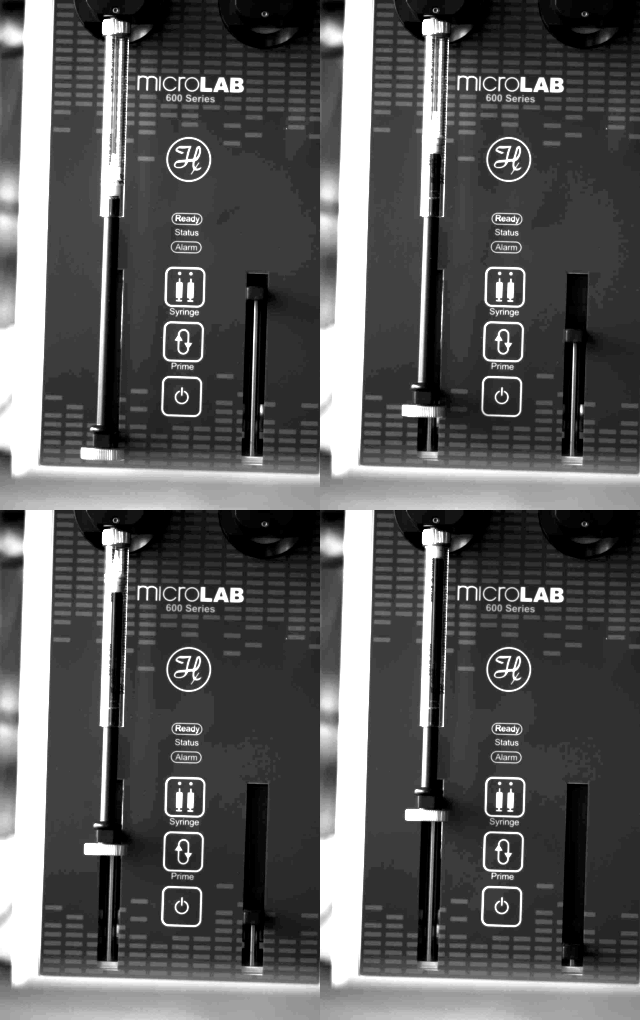
\includegraphics[width=0.8\textwidth]{images/combined}
    \end{center}
    \vspace{-1.2em}
  \caption{Cycling behaviour}
\end{figure}
\begin{multicols}{2}
    \lipsum[2]
% \begin{figure}[H]
%    \begin{center}
%    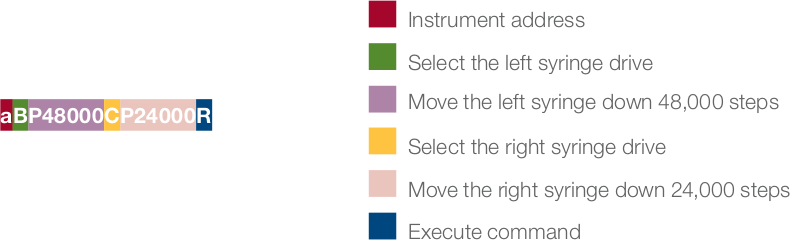
\includegraphics[width=0.45\textwidth]{images/examplemanualcommand}
%    \end{center}
%    \vspace{-1.2em}
%  \caption{Example syringe movement command string}
%\end{figure}
\end{multicols}
\end{posterbox}

%%%% Column 3 %%%%%%%%%%%%%%%%%%%%%%%%%%%%%%%%%%%%%%%%%%%%%%%%%%%%%%%%%%%%%%%%%%
%----------------------------------------------------------------------------------------
%	EDM SCREENS
%----------------------------------------------------------------------------------------
\begin{posterbox}[name=edmscreens,column=3]{EDM Screens}
    The EDM screens allowed users to access the cycling commands and view the output of status/error requests.
    A bar chart was used to depict the amount of liquid in the syringes. Updates to this bar chart created an
    "animation" effect that would let users know when the syringes are picking up or dispensing fluid. The
    change in the syringe position also triggered the appearance of an arrow that indicates if the syringe is
    picking up or dispensing.
\end{posterbox}
%----------------------------------------------------------------------------------------
%	EDM IMAGE
%----------------------------------------------------------------------------------------
\begin{posterbox}[name=edmimage,column=3,below=edmscreens,headerfont={},headershape=rounded,boxheaderheight=0em,boxColorOne=white,borderColor=white]{rounded}
\begin{figure}[H]
\begin{center}
\vspace{-1em}
\setlength{\fboxrule}{2pt}
\fbox{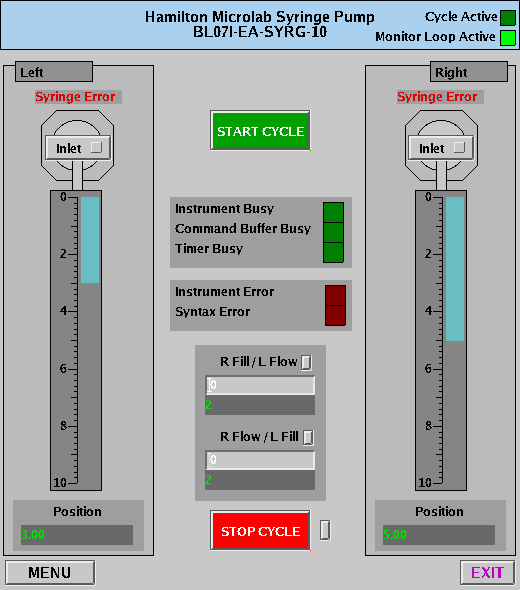
\includegraphics[width=0.73\textwidth]{images/cycleedm}}
\caption{EDM screen for controlling syringe cycling}
\vspace{-1.2em}
\end{center}
\end{figure}
\end{posterbox}
%----------------------------------------------------------------------------------------
%	OUTCOME
%----------------------------------------------------------------------------------------
\begin{posterbox}[name=outcome,column=3,below=edmimage]{Outcome}
The cycling behaviour was unable to run overnight without issue. However, some instrument error requests would
give misleading information. The responsiveness of some of the information on the EDM screen was also
    dependent on the number of information requests being sent to the device. To syringe positon and related
    information were given their own seperate monitor loop to counteract this. While this created a bit of an
    improvement, syringe movements that were too fast would often get "missed" by the loop. 
\end{posterbox}
%----------------------------------------------------------------------------------------
%	FUTURE WORK
%----------------------------------------------------------------------------------------
\begin{posterbox}[name=futurework,column=3,above=bottom]{Future Work}
 \begin{itemize}
    \item Write a simulation for the syringe pump
    \item Add a cleaning command to the library with a corresponding button on the EDM screen
    \item Allow the EDM screen to update immediately when the syringe volume is changed
    \item Accomodate daisy-chaining multiple syringe pumps
\end{itemize}
\end{posterbox}

\end{poster}
\end{document}
